% Chapter 1

\chapter{Introduction} % Write in your own chapter title
\label{Introduction}
%\addtotoc{Introduction}
\lhead{\emph{Introduction}} % Write in your own chapter title to set the page header

\section{3D Optical Network-on-Chip}
\subsection{3D Network on-chip}
\subsection{Nanophotonics interconnects technology}
Natural resource nowadays is the motivation for many researches on energy management in buildings and homes. Energy management is not only the reduction of energy consumption but also the balance between energy consumption and energy generation. 
Smart Grid (SG) and Smart Building Automation (SBA) are the approaches that have the main impact on energy saving issues. 

The concept of SG is associated with the energy production side~\cite{smartgrid}. Concretely, the \textit{grid} refers to the electric grid or a network of transmission lines, substations, transformers and other components that deliver the electricity from the power plants to the consumers. Meanwhile, modern energy management techniques and communication infrastructures such as Internet, wireless communications or Power-Line Communications (PLC)  make the \textit{grid} smart with the possibility of automated monitoring, computing, controlling without human intervention~\cite{Galli5622060,Galli5768099,Gungor6011696,Berger2013}. In addition, the purpose of SG also includes the integration of large-scale renewable energy systems such as wind power along the farms or solar power on the top of buildings  in order to protect the environment and ecosystem, instead of using only the  energy generated by the traditional power plants, e.g. hydro power, thermal power or nuclear power. 

In contrast, in SBA as in Figure~\ref{fig:I1}, the principle problem is how to reduce the energy consumption inside homes or buildings. A smart building can be achieved by the generation and efficient usage of energy. The modality of energy usage comes from subsystems such as lighting system, office equipment, Heating, Ventilation and Air Conditioning (HVAC), etc. Therefore, the energy waste elimination effort can concentrate on these systems by sensing and automatically fluctuating their power to adapt to the environment condition. In a smart system, human intervention must be restricted, the automation system automatically control the equipment through such a Energy Management System (EMS). Similar to SG, in SBA, the communication infrastructure plays an important role in exchanging the information among the components inside the EMS. That is the reason why PLC and Wireless Sensor Networks (WSN) can be considered as potential solutions for environment monitoring and subsystem fluctuation, but WSN is more promising because of its flexibility and low cost. With WSN, the sensors capture the environmental parameters and report data to the EMS center through wireless transceivers. The control center, with the information about the state of subsystems, then fluctuates their power consumption to adapt to the environmental variation. 
\begin{figure}
\centering
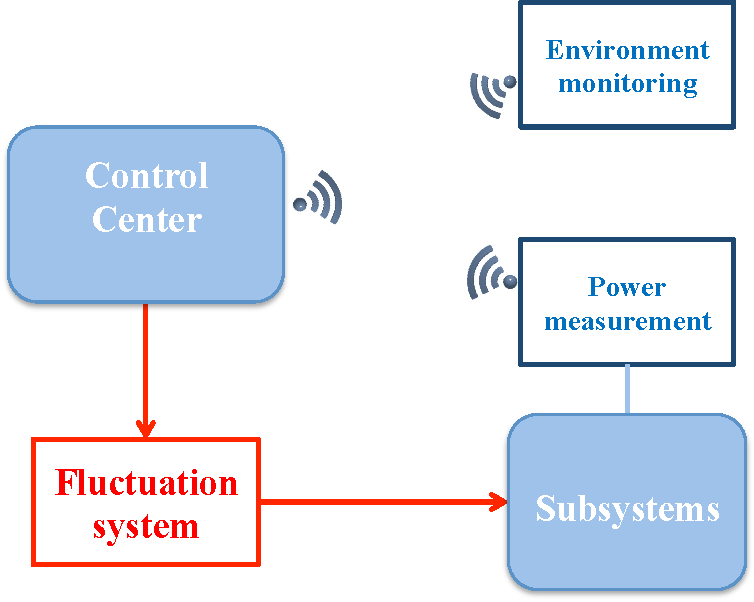
\includegraphics[width=0.6\textwidth]{./chapters/chapter1/images/SBA.pdf} 
\caption{Principle components of a SBA system.} 
\label{fig:I1} 
\end{figure}

The monitored environmental parameters can be occupancy, light intensity, temperature, moisture, sound, etc. Detecting and analyzing these information allows the system to automatically regulate the equipment to comfort the users, especially with the devices requiring time to start up such as HVAC system, and to regulate the power consumption. Except for occupancy, other types of environment can be easily monitored by the corresponding sensors such as light sensors, temperature sensors, humidity sensors, microphones, etc. Meanwhile, the occupancy detection is an interesting subject for many recent researches~\cite{Agarwal11ACM,Weng12DTC,Agarwal10BuildSys,Lu10ACM}. The occupancy can be detected directly by a Passive Infrared Sensor (PIR) or camera~\cite{Weng12DTC,Agarwal11ACM,Agarwal10BuildSys}, or indirectly by analyzing the events happening inside house or building, e.g. door state, variation on the total power signal~\cite{Chen13ACM}, abnormally increase of  the CO2 concentration~\cite{Wang01111999}.
For example, a couple of magnetic Reed Switch (RS) door sensor and PIR sensor can be used to detect the occupancy in offices or rooms~\cite{Agarwal11ACM,Weng12DTC}. Although PIR sensors are the most ubiquitous form for motion sensing, it is not enough for occupancy detection because people inside rooms/offices tend to maintain their posture when working in front of a computer, watching television or sleeping. To overcome this challenge, combining with an RS door sensor, which can determine if the door is open or closed, is more efficient. 
\begin{figure}
\centering
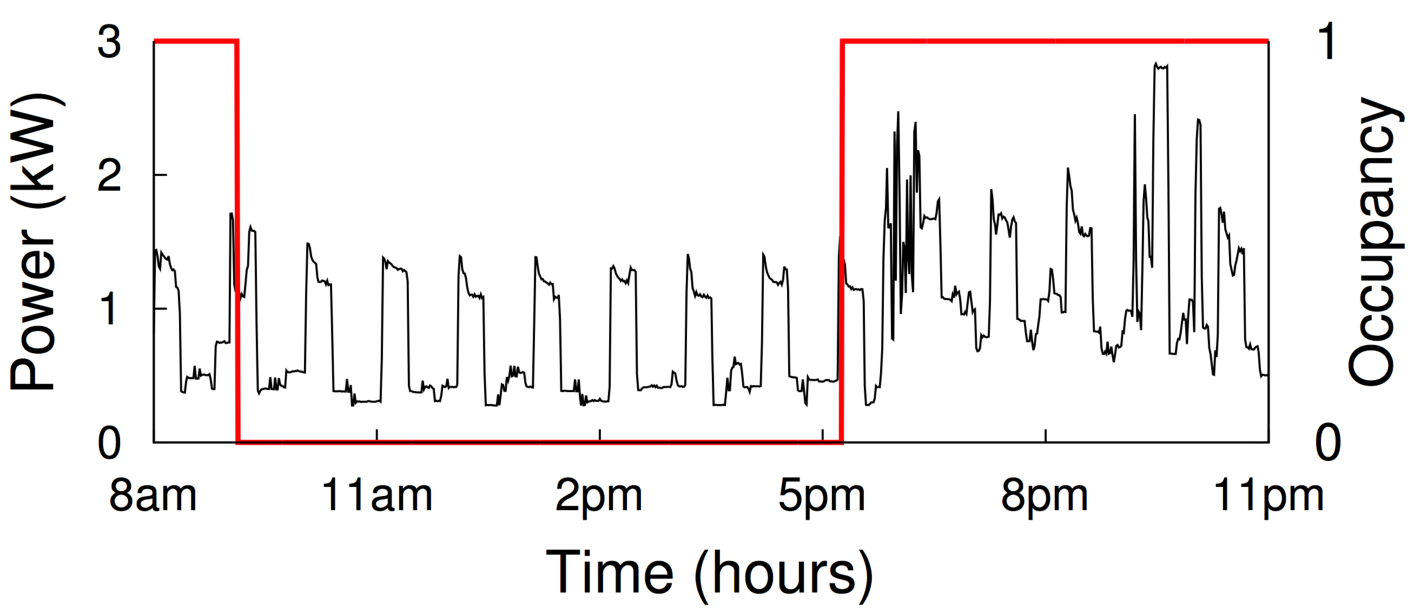
\includegraphics[width=0.7\textwidth]{./chapters/chapter1/images/nonintrusive_occupant_power.pdf} 
\caption{Variation on the power signal when the occupant turns on some devices~\cite{Chen13ACM}.} 
\label{fig:I2} 
\end{figure}
%---------------------------------
Another example of occupancy monitoring is to detect the large changes on the aggregate power signal and infer the occupancy~\cite{Chen13ACM}. As shown in~Figure~\ref{fig:I2}, the background load frequently appears and does not imply the occupancy. This load is derived from the presence of the devices driven by an automated controller such as fridge or HVAC system. When having the presence of the occupants, their physical interactions with loads such as switching on the lamp, turning on the television, etc., will imply changes on the power signal.
The large changes can be detected by comparing the average power, standard deviation or power range in a sliding window of signal with corresponding thresholds. Obviously, the accuracy of this monitoring system strongly depends on the survey of background load due to the variation of this parameter according to the time of day and year such as day or night, spring or winter.
Besides, the state transition of some types of devices can also provide the interaction of users~\cite{Ridi15}. For example, a washing machine has five states including off, wash, rinse, spin and maintenance wash, the user interaction can make the transition from the first to the second state.

In SBA, besides the environment monitoring, the power consumption of the equipment also needs to be measured and reported so that the control center can make a suitable fluctuation to adapt to the environmental variation.


\section{Thesis contributions}
%\subsection{Intrusive Load Monitoring}
Similar to the environment monitoring sensors, power measurement units also require a wireless protocol to communicate with the control center. Power metering can be implemented by two ways: intrusive and non-intrusive. In intrusive approach, the measurement is deployed at each individual equipment. In contrast, the Non-Intrusive Load Monitoring (NILM) \footnote{sometimes also referred as NIALM (Non-Intrusive Appliance Load Monitoring) or Electrical Load Disaggregation} can detect and estimate the power consumption of all devices on the monitored branch circuit with only one power meter installed on the main power entry~\cite{Hart92}. Intuitively, non-intrusive approach helps to reduce the deployment cost but requires a long period of observation to analyze the power characteristics of each device. 

As shown in Figure~\ref{fig:I3}, an Intrusive Load Monitoring (ILM) system can be implemented in a direct of indirect method. The direct one attaches a power meter to each device. Therefore, direct ILM obviously performs with high accuracy but has some disadvantages such as high cost and interruption on the power supply to install the meters. In contrast, the indirect method uses low-cost sensors to detect the measurable signals emitted by the device to estimate the power consumption. For example, a light sensor can detect the power state of a television and infer the corresponding consumed energy, an acoustic sensor can be applied to recognize the operation of the fridge compressor~\cite{Kim09Ubicomp}. 

\begin{figure}
\centering
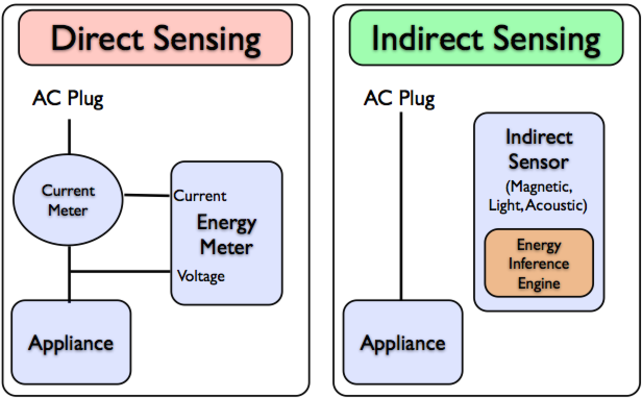
\includegraphics[width=0.8\textwidth]{./chapters/chapter1/images/direct_indirect_sensing.pdf} 
\caption{Direct and indirect power measurement \cite{Kim09Ubicomp}.} 
\label{fig:I3} 
\end{figure}
%---------------------------------




%\subsection{Non-Intrusive Load Monitoring}\label{nilm}

In contrast with intrusive approaches, the non-intrusive ones rely on only one power meter at the main power supply. An NILM algorithm tries to extract some specific features from the aggregate power signal to identify the corresponding devices.
Assuming there are $N$ devices connected to a unique power meter, each device $i\in \{1,\ldots, N\}$ can operate at one state $j$ of $m_i$ modes, which consumes a power of $w_{ij}$, $j \in \{1,\ldots,m_i\}$. Denote $s_{ij}(t)$ as the Boolean indicator of state $j$ of device $i$ at time $t$:
\begin{equation*}
s_{ij}(t)=\begin{cases}
1 \mbox{ if device $i$ operates at state $j$}\\
0 \mbox{ otherwise}.
\end{cases}
\end{equation*}
The aggregate power consumption can be represented as follows:
\begin{equation}\label{eqI6}
x(t)=\sum_{i=1}^{N}{\sum_{j=1}^{m_i}{s_{ij}(t)\times w_{ij} + e(t)}},
\end{equation}
where $e(t)$ is a noise or error term. From this model, the vector $\mathbf{s}$ containing all state indicators $s_{ij}$, $i=1,\ldots,N, j=1,\ldots,m_i$ of the devices from $1$ to $N$ can be determined by solving the following minimization problem:
\begin{equation}\label{eqI7}
\hat{\mathbf{s}}(t)=\argmin_{\mathbf{s}(t)}{\parallel x(t) - \sum_{i=1}^{N}{\sum_{j=1}^{m_i}{s_{ij}(t)\times w_{ij}}} \parallel_d},
\end{equation}
where $\parallel.\parallel_d$ denotes the $l_d$ distance. In the context of NILM, we can use some distance metrics such as $l_1$, $l_2$.
This problem is computationally intractable and impractical to be exactly solved by exhaustive techniques unless $N$ is small. Instead, heuristic algorithms might be considered. There are three principles for any NILM algorithm, including:
\begin{itemize}
\item Select and mathematically characterize the specific features or signatures.
\item Deploy the suitable hardware  to measure the desired signal.
\item Develop an algorithm to detect those features/signatures from the signal.
\end{itemize}
The characterization of features and signatures needs the knowledge on the operation states of the devices, which can be categorized into four types, as surveyed in \cite{Zoha12}, including:
\begin{itemize}
\item Type-I: devices with two states (ON/OFF) such as lamp, toaster, etc.
\item Type-II: finite state machines with a finite number of operation states, e.g. washing machine, stove, etc.
\item Type-III: continuously varying devices with variable power consumption such as power drill or dimmer lights.
\item Type-IV: devices that remain active throughout days or weeks and consume a constant level of power such as smoke detector, internet modem, etc.
\end{itemize}
The three first categories are proposed by \cite{Hart92} and shown in Figure~\ref{fig:I4}, while the last one is highlighted in \cite{Zeifman11TCE,Baranski03}. Besides, the selection of features/signatures also depends on the sampling frequency of meters and can be divided into two groups: low frequency  and high frequency.
Algorithms based on low-frequency signal focus on detecting the steady-state features such as average power, step-changes, etc., while high-frequency hardware allows us to identify the devices from the transient phase and harmonics.
\begin{figure}
\centering
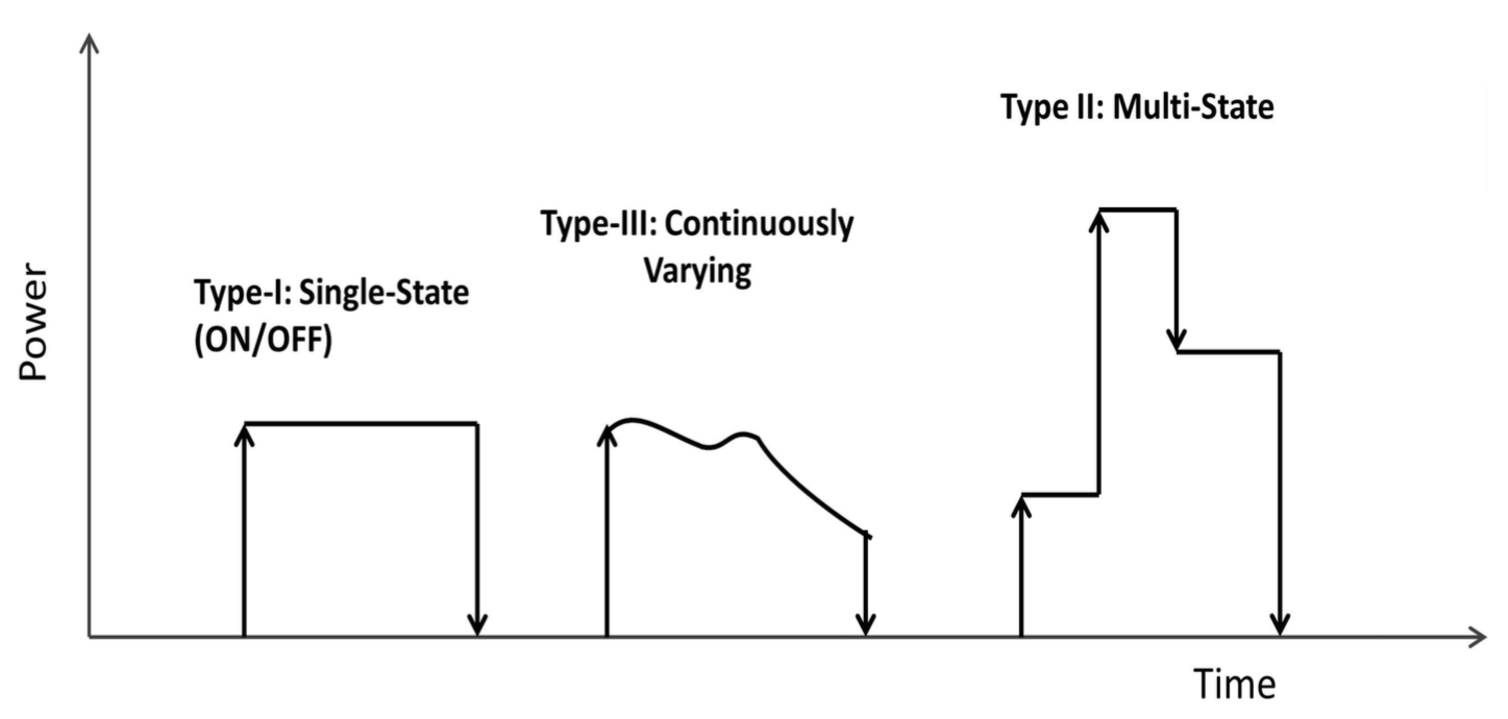
\includegraphics[width=0.8\textwidth]{./chapters/chapter1/images/load_categories.pdf} 
\caption{Different categories of load based on energy patterns \cite{Zoha12}.} 
\label{fig:I4} 
\end{figure}

%\subsection{Hybrid Load Monitoring}
A hybrid approach between intrusive and non-intrusive load monitoring, called Hybrid Load Monitoring (HLM), was proposed in recent years~\cite{TangW16,Berges10,Berges11,Guvensan13,Uddin12}. In this approach, a sensor network is deployed in homes to monitor the environmental parameters such as acoustic noise, light intensity, occupancy, etc., to detect the operation of some specific devices. The difference between the hybrid and intrusive approaches is that the sensors are only installed to monitor a part of all devices while the others are still identified by an NILM algorithm with aggregate power measurement. Therefore, HLM allows for a reduction of the cost of the intrusive approach and an increase of the detection accuracy of the non-intrusive one. In the context of this thesis, we will focus on hybrid methods in order to improve the performance of the existing NILM algorithms.


\section{Dissertation Organization}

\textbf{Chapter 2: State of the art}\\
This chapter reviews the techniques and approaches used in load monitoring, from intrusive to non-intrusive and from low frequency to high frequency sampling hardware. 
In intrusive approach, each device is attached to a set of sensors, which detect the environmental variation generated by the device and infer its power state. Although this approach shows a high accuracy, it is difficult to deploy in smart homes and buildings because of high cost and too much technical intervention on the infrastructure. 
Instead, by using only one power meter at the main entry of electricity, non-intrusive approach is more promising to study. In this approach, the electrical features of each device are characterized and an algorithm is developed to extract the features from the aggregate power load and therefore to identify the corresponding device.
The selection of electrical characteristics depends on the sampling frequency of hardware. Concretely, low frequency hardware is suitable for the stable loads with the features related to the average power demand, rising step-changes, falling step-changes, etc., while high frequency hardware is more efficient to identify the devices based on the transient signal and harmonics analysis. 
In recent years, a hybrid approach of intrusive and non-intrusive is studied, in which the sensors can be deployed to detect the state of several devices, while the rest is still recognized by a non-intrusive algorithm.

\textbf{Chapter 3: $l1$-norm minimization based algorithms for NILM}\\
In this chapter, the minimization problem in NILM is solved by directly using the brute force method to determine the state of each device. In this method, all possible combinations of operating devices are in turn applied to calculate the absolute error between their total power demand and the measured aggregate power. The set of devices giving the minimum error are identified as running. However, if there is more than one device having the same power demand, the detection is no more accurate. The main contribution of this chapter is to propose two solutions to overcome this challenge and to improve detection accuracy, including:
\begin{itemize}
\item Difference-based algorithm to compare the difference between the current state and the previous state of each device.
\item Probability-based algorithm to use the state transition probability to decide the operating devices.
\end{itemize}
An experiment is also implemented with a small set of devices installed our laboratory.

\textbf{Chapter 4: SmartSense: Sensor-Aided NILM}\\
The main contribution of this thesis, SmartSense system, is presented in this chapter. To improve performance of NILM algorithms, we propose to use the operating probability of each device as an external information. The probability can be estimated from a sensor network. Different from the intrusive approach, only a small subset of some devices are selected to be monitored by the sensors while the others are assumed to be equiprobable among the states. Although it could be perceived as similar to a hybrid approach, however, instead of identifying the state of devices from the sensor signals, we transform this state to a probability and an NILM algorithm can still be applied to all devices combined with this external information. Therefore, monitoring a set of devices can help to improve the detection of the others. The algorithms applied to SmartSense in this thesis include:
\begin{itemize}
\item Compositional Pareto-algebraic Heuristic.
\item Dynamic Programming.
\item Edge Detection.
\item Dynamic Time Warping.
\end{itemize}

These proposed algorithms are applied to both our own dataset as well as publicly available dataset. The evaluation of performance improvement is given in \textbf{Chapter 5: Experimental results}. Meanwhile, the conclusions and perspectives of this thesis will be presented in \textbf{Chapter 6: Conclusions and perspectives}.
